%*****************************************
\chapter{A System}\label{ch:a_system}
%*****************************************

\section{System Overview}

Building a machine that demonstrates the general intelligence required
for commonsense reasoning is a longstanding goal of the field of
artificial intelligence.  There have been many approaches to building
a machine that demonstrates general intelligence, some are based on
logical representations, others are based on large collections of
statistical knowledge, while still others approach the problem by
learning everything from scratch from the physical world.  I see the
problem as requiring a combination of many different types of
representations and reasoning processes.




\subsection{Reflectively Traced Frame Memory}

Procedural tracing can be thought of as enabling a part of an
interpreter that checks for important events as a process runs.  This
ability can be used to trace the temporal order of events, i.e.
generating a trace, or to otherwise organize or summarize events in a
more useful way that can be used by other procedures, either
concurrently or after the fact.  Having this ability built into the
memory system, allows keeping track of the provenance of information as
it is written and read.  This ability is built into all structures in
the architecture, so if any tracing of data provenance is required at
any time for any object, this ability can be enabled.

At higher levels, these procedural tracing events result in event
streams that can be listened to by multiple concurrent processes that
each allocate iterators for a stream.  As a concurrent process
increments its iterator, it reasons about the event that has occurred
in the object memory, and the result of this reasoning is the creation
of meta knowledge in a causally consistent knowledge base.  This is an
example of the "glom" theory of cognitive evolution, where cognitive
abilities are added on top of previous cognitive abilities without
changing the underlying functionality.  I've used procedural tracing
to maintain multiple consistent representations for the same
knowledge.

When a plan fails, I need to correct the knowledge that generated that
plan.  When multiple processes are adding knowledge to the same
knowledge base, it becomes important to keep track of the provenance of
this knowledge, when I need to make distinctions between situations
that appear identical.  If I need to learn a new rule for
categorization of situations, or even a new category entirely, I need
to go back to the correct features and processes that performed those
categorizations of the identical situations that I need to further
distinguish.

\subsection{Efficiency Problems with Reflective Tracing}
\label{sec:reflective_tracing}

There are serious efficiency problems that must be carefully
sidestepped when one is dealing with reflective knowledge.  For
example, infinite reflection loops result in an infinite processor and
memory consumption pattern, after only a single change to a knowledge
representation.  The solution to this problem is to have various means
of controlling the reflective tracing focus.  I will discuss the
various methods for controlling the tracing focus of the reflective
memory that I have found useful in the development of my system in
Section~\ref{sec:methods_for_focusing_reflective_tracing}.


\subsection{Methods for Focusing Reflective Tracing}
\label{sec:methods_for_focusing_reflective_tracing}
\marginpar{Section~\ref{sec:methods_for_focusing_reflective_tracing}
  is referenced from Section~\ref{sec:reflective_tracing}.}


\subsection{Procedural Tracing}

The idea of having procedural tracing at the operating system level is
important because it does allow all programs running on the operating
system to assign credit to processes when bugs do occur.

%TS>> then you have to refer to the robust os literature and talk about their methods for
%TS>>tracing and justify it with their literature and then show how yours adds to it and 
%TS>>defend it against and in that community... ....might be a distraction .....
%TS>operating system... seems pretty general... how bout in the" memory's working set"

Although it is important to have protected memory boundaries between
programs for reasons of security, privacy, and stability, having good
ways for processes that do share memory to trace the provenance of
individual memory events, allows for much tighter and intelligent
interaction between all processes in the entire system.
        

\subsection{Trace Only an Appropriate Level of Abstraction}

It does not make sense to trace below a certain depth of processing.
If I were to trace all of the lowest level details of execution at
all times, there would be no way to take advantage of that amount
of detailed information.

There are barriers in my system for only allowing tracing to occur for
specific parts of the code.  The ability to focus the tracing of object
usage allows the possibility of tracing either high or low-level events
in a uniform manner.

\subsection{Keeping Tracing from Taking Too Much Time and Storage}

When a set of objects are out of the focus of tracing, these objects run
operate at full speed and do not increase the memory usage of the
tracing component.  There is a new proposal by McCarthy to build a new
programming language that remembers everything that it does; it is
called Elephant 2000 \citep{mccarthy:1994}.


\section{An Operating System and a Programming Language}

I've written a multi-core operating system, including a compiler and a
programming language, on top of this traceable and distributed memory
layer \citep{morgan:2009}.

Because the system is meant to combine many artificial intelligence
techniques, I have tested my platform running thousands of parallel
processes concurrently on an 8-core machine.  These processes can
control and watch one another execute.  I feel that the field of AI
is not separate from the low-level details of software engineering,
and my project embodies that philosophy.

Many people see AI as being a purely theoretical and mathematical
field, and I strongly disagree.  I need good software engineers in
order to solve most of the problems I face in getting these massive
software systems to work together.

I have built a layered cognitive architecture on top of my custom
operating system, programming language, and compiler.

\subsection{Why not use Lisp?}

Lisp is a great programming language.  I wrote a custom programming
language for the project and didn't use lisp.  Lisp simply isn't fast
enough, and isn't very well supported; when you find a bug in a lisp
compiler, it is difficult to find the support to fix the bug.  I wrote
the first version of the reflectively traced memory system in lisp and
realized that Steele Bourne Common Lisp had memory bugs when the
system grew beyond 600 megabytes of RAM.  Allegro Lisp is a commercial
solution, but it costs many hundreds of dollars for their commercial
compiler, and I feel strongly against having that commercial
requirement for building academically intentioned open-source
software.  The main problem with lisp is it's lack of speed and lack
of support, so I found myself writing a lot of C extensions even when
programming in Lisp.  C is good for speeding up inner loops of
algorithms as well as necessary for interfacing with the Linux, Mac,
or Windows operating systems, which are all written in C.

\section{A Layered Cognitive Architecture}

Further, I have developed a cognitive architecture within my
language that provides structures for layering reflective processes,
resulting in a hierarchy of control algorithms that respond to
failures or other events in the layers below.


\subsection{Perceptual Support of Physical Knowledge}

\begin{figure}[bth]
  \center
  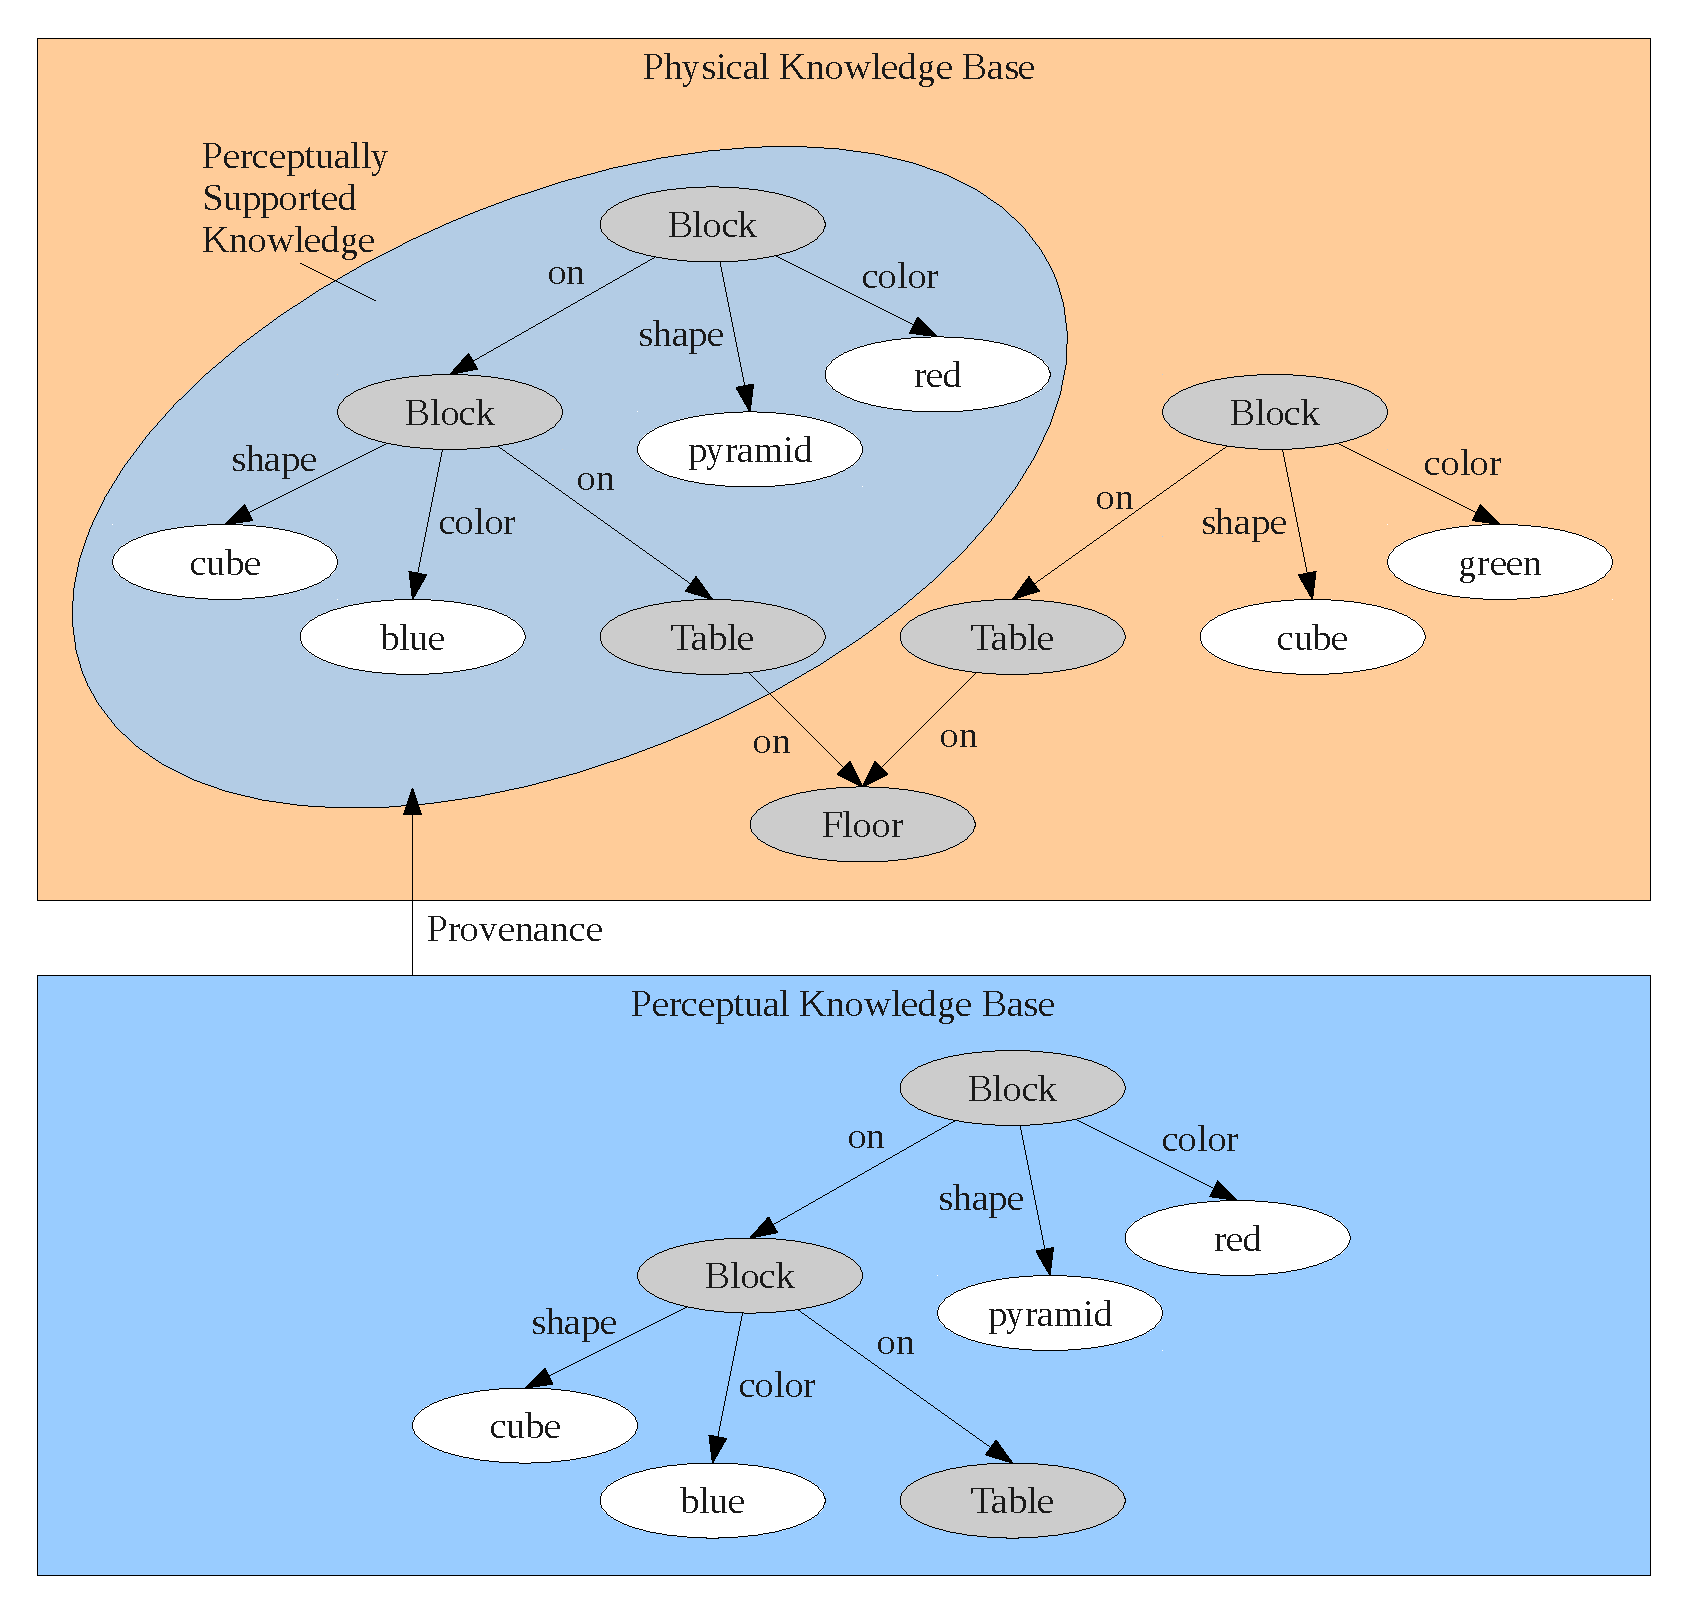
\includegraphics[width=10cm]{gfx/physical_perception}
  \caption[Perceptual provenance provides support for physical knowledge]{Perceptual provenance provides support for physical knowledge.}
  \label{fig:physical_perception}
\end{figure}

See Figure~\ref{fig:physical_perception}.


\subsection{A Serial Process Representation}
\label{sec:serial_process_representation}

\begin{table}
  \myfloatalign
  \begin{tabularx}{\textwidth}{XllllX}
    & [prog & [pick-up & `red   & `cube]    & \\
    &       & [put-on  & `blue  & `cube]    & \\
    &       & [pick-up & `green & `pyramid] & \\
    &       & [put-on  & `red   & `cube]]   & \\
  \end{tabularx}
  \caption[Representation of a serial process]{Representation of a serial process.}
  \label{tab:serial_process_representation}
\end{table}

A representation of a serial process is shown in
Table~\ref{tab:serial_process_representation}.  This representation is
an ordered tree symbolic representation, which is capable of
representing any Lisp-like expression in my language interpretter.

\subsection{A Parallel Process Representation}
\label{sec:parallel_process_representation}

\begin{table}
  \myfloatalign
  \begin{tabularx}{\textwidth}{XlllllX}
    & [prog & [parog & [use-left-hand-to-pick-up  & `red   & `cube]    & \\
    &       &        & [use-right-hand-to-pick-up & `green & `pyramid] & \\
    &       & [parog & [use-left-hand-to-put-on   & `blue  & `cube]]   & \\
    &       &        & [use-right-hand-to-put-on  & `red   & `cube]]]  & \\
  \end{tabularx}
  \caption[Representation of two serial parallel processes]{Representation of two serial parallel processes.}
  \label{tab:parallel_process_representation}
\end{table}

See Table~\ref{tab:parallel_process_representation}.


\subsection{Details of Inferring the Effects of a Plan}
\label{sec:details_of_inferring_the_effects_of_a_plan}
\marginpar{Section~\ref{sec:details_of_inferring_the_effects_of_a_plan}
  is referenced from Section~\ref{sec:inferring_the_effects_of_a_plan}.}



\subsection{Goal-Oriented Action Hypothesis Generation Techniques}
\label{sec:goal_oriented_action_hypotheses_generation_techniques}
\marginpar{Section~\ref{sec:goal_oriented_action_hypotheses_generation_techniques}
  is referenced from Section~\ref{sec:goal_oriented_action_hypotheses}.}


\subsection{Debugging Plans by Reflectively Tracing the Provenance of Knowledge}

I trace the procenance of knowledge from perceptual knowledge as it
is manipulated into other knowledge representations, driven by a
goal-oriented learning algorithm.  Normally, when plans fail, rule
learning is used to update beginning and ending condition transition
function hypotheses for actions relative to various knowledge bases.

In many systems, when these plans fail, it is often unclear which part
of the plan was responsible for the failure.  In the simplest cases, a
specific low-level action may have been executing, which implies that
precondition categories were incorrectly mapped to postconditions or
the range of postconditions was not broad enough.  In the worst cases,
it is impossible to tell what part of the plan failed because the plan
is such a complicated tangle of compiled numbers that the only
recourse is to nudge a few of these numbers using hill-climbing toward
an average of a universal goal.  Rethinking this problem with my new
approach that maintains provenance for knowledge used in creating
plans allows debugging the complex web of goal-oriented knowledge, and
reflectively, also manipulating the processes involved in creating
that knowledge.



